\vspace{10pt}
\section{Modeling of the Cross-Point Memory}\label{sec:model}

In this section, a detailed mathematical model of cross-point memory array is built. By using the proposed model with specific parameters and
boundary conditions, different read/write schemes can be easily evaluated
at the very early stage of the design.

\subsection{Basic model of Cross-Point Memory}
Figure.~\ref{fig:modeling} shows the circuit model of the $M$ by $N$ cross-point ReRAM array. The horizontal lines are word lines and vertical lines represent the bit lines. The ReRAM cells are located at each cross point of one word line and one bit line. The resistance of the ReRAM cell at the cross point of the $i^{th}$ word line and $j^{th}$ bit line is indicated as $R_{i,j}$. We assume the resistance of the interconnect nanowires between two adjacent cross point has the same value of $R_{line}$. The input resistance of each word line and bit line is $R_v$ and the resistance of sense amplifier is $R_s$. In order to set up the Kirchhoff's Current Law (KCL) equations, the voltage at each cross point is indicated as $V_{i,j}$ for word line and $V'_{i,j}$ for bit line. A detailed cross point is also shown in Figure.~\ref{fig:modeling}. Besides, the input voltage for the $i^{th}$ word line is $V_{Wi}$ and for the $i^{th}$ bit line is $V_{Bi}$. In the case of two side voltage input of word line, the voltage at the other end of the $i^{th}$ word line is denoted as $V_{W1}$. Finally, the voltage at the sense amplifier is $V'_{Bi}$ during the read operation.

\begin{figure}%[!hb]
\centering
  % Requires \usepackage{graphicx}
  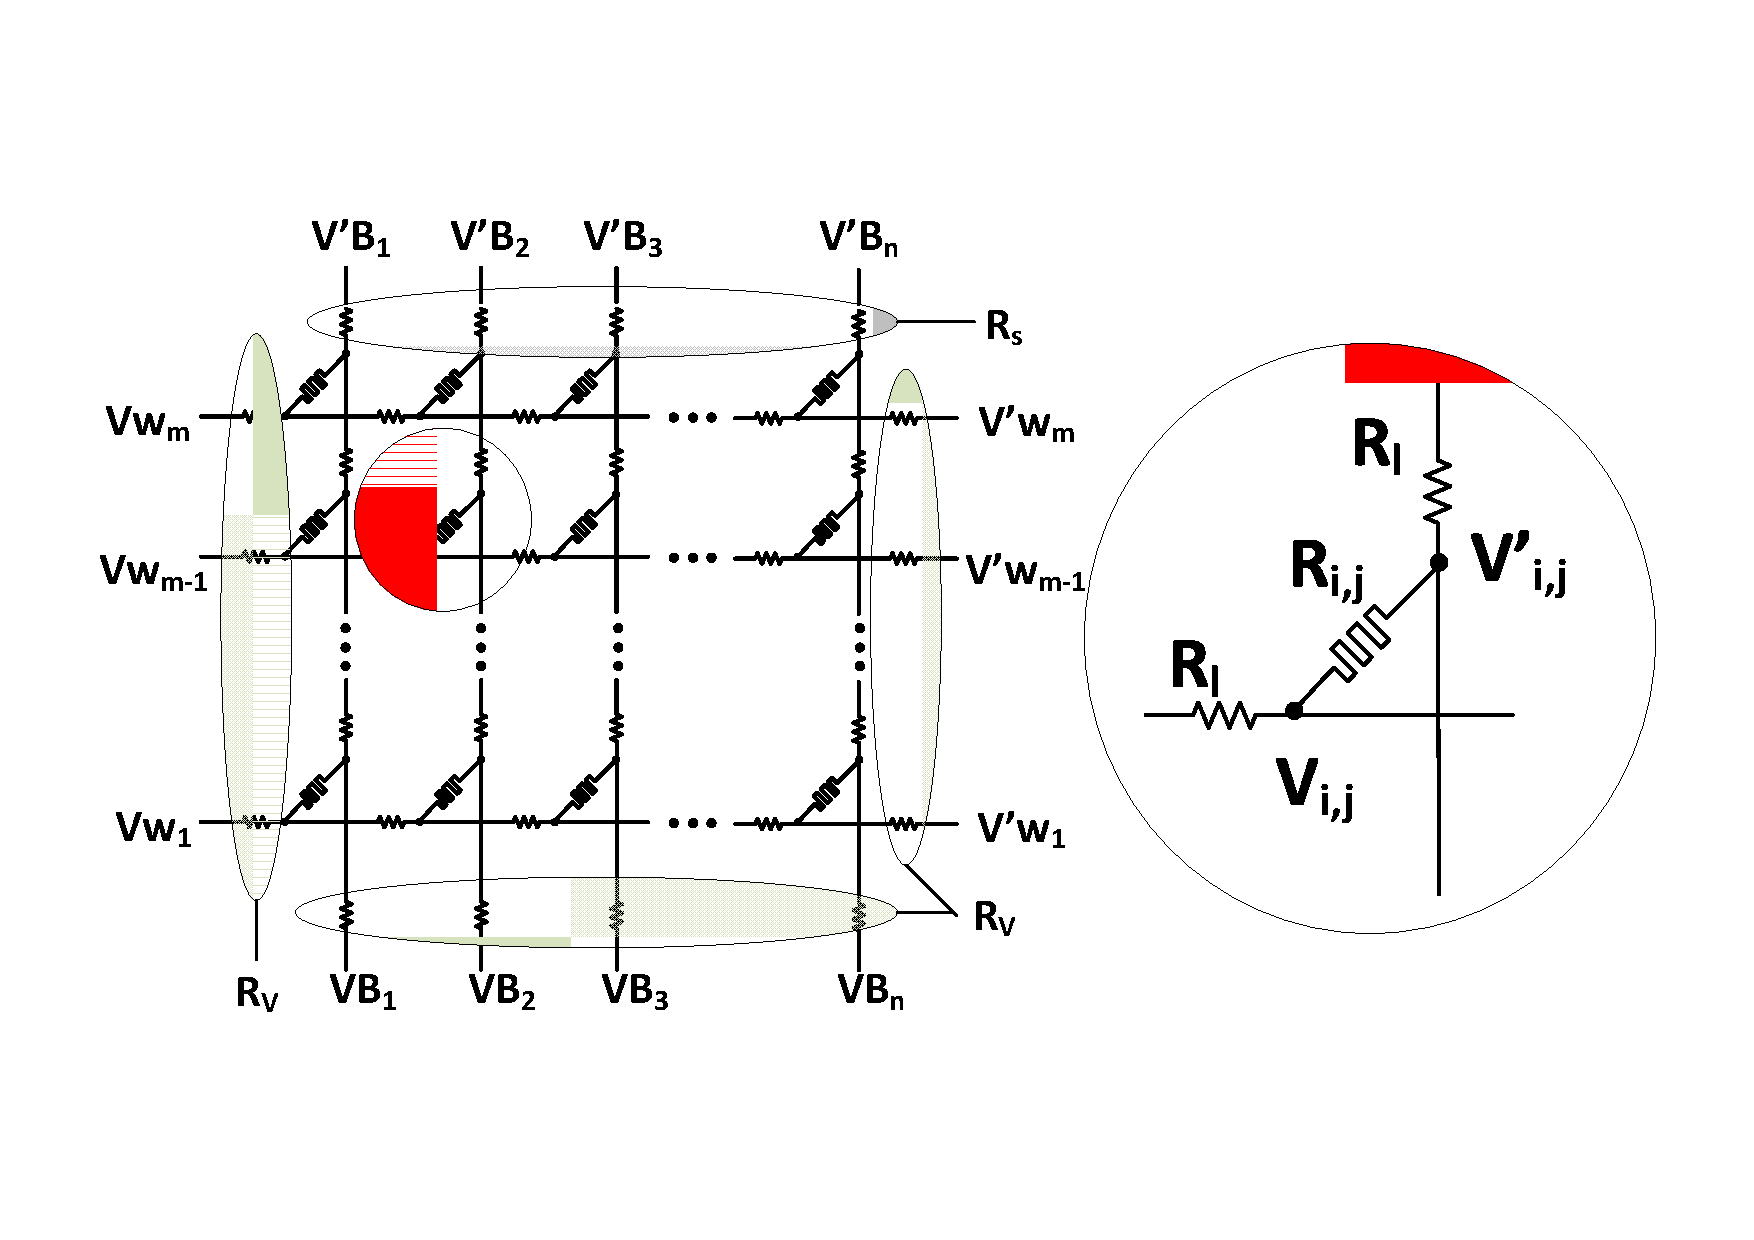
\includegraphics[width=0.45\textwidth]{./figures/model_reverse.pdf}\\
  \caption{The basic model of typical cross-point array.}\label{fig:modeling}
\end{figure}
\subsection{Mathematical Model of the Cross-Point Array}
Based on the circuit model, the current equation for each cross point can be built following the KCL:
\begin{equation}
  {\Sigma}_{I=1}^kI_k=0.
\end{equation}
All of the cross points have similar structure with no more than three current injection and therefore it is easy to set up the KCL equation for each cross point. However, we should treat the cross points at the edges of the array seriously because there are different conditions for different write/read schemes. For example, the unselected word line for write operation can be either half biased or left floating. Thus, the edge conditions should be adjusted according to each write/read schemes. However, even consider the different conditions of at the edge of the array, all of the cross points can be classified into three major categories: Normal point, Activated point and Floating point.

The normal points located inside the memory array. In other words, for all of the nodes with $1<i<m$ and $1<j<n$, the KCL equations take the form of
\begin{equation}\label{equ:KCL1}
R_l^{-1}V_{i,j-1} -(2R_l^{-1}+R_{i,j}^{-1})V_{i,j}+ R_l^{-1}V_{i,j+1}+R_{i,j}^{-1}V'_{i,j}=0,
\end{equation}
for the node at word line layer and
\begin{equation}\label{equ:KCL2}
R_l^{-1}V'_{i-1,j} -(2R_l^{-1}+R_{i,j}^{-1})V'_{i,j}+ R_l^{-1}V'_{i+1,j}+R_{i,j}^{-1}V_{i,j}=0,
\end{equation}
for the node at bit line layer.

The activated point and floating point represent the node at the edge of cross point array with different conditions: an edge point, which have been directly connected to the voltage input or the ground, can be considered as a activated point. Otherwise, it is a floating point. Take the point located at the intersection of $i^{th}$ word line and $1^{st}$ bit line for example. If the $i^{th}$ word line is activated by a voltage input of $V_{Wi}$, then this cross point is an activated point, and the KCL equation for this point is:
\begin{equation}\label{equ:KCL3}
-(R_v^{-1}+R_l^{-1}+R_{i,1}^{-1})V_{i,1}+ R_l^{-1}V_{i,2}+R_{i,1}^{-1}V'_{i,1}=-R_v^{-1}V_{Wi},
\end{equation}
otherwise, it is left floating and has the KCL equation take the form of
\begin{equation}\label{equ:KCL4}
-(R_l^{-1}+R_{i,1}^{-1})V_{i,1}+ R_l^{-1}V_{i,2}+R_{i,1}^{-1}V'_{i,1}=0.
\end{equation}

For the reasons of clarity, a vector ${V}_{2mn\times 1}$ is used to represent all of the variables in the KCL equations:
\begin{equation}\label{equ:V1}
{V}=[{V_1}^T,{V_2}^T...{V_m}^T,{V'_1}^T,{V'_2}^T...{V'_m}^T]^T,
\end{equation}
where,
\begin{equation}\label{equ:V2}
{V_i} = [V_{i,1},V_{i,2}...V_{i,n}]^T,\\
\end{equation}
\begin{equation}\label{equ:V3}
{V'_i} = [V'_{i,1},V'_{i,2}...V'_{i,n}]^T.
\end{equation}

Then the KCL equations can be considered as a system of linear equations and has the form of
\begin{equation}\label{equ:matrix}
A_{2mn\times{2mn}}\cdot V_{2mn\times{1}} = C_{2mn\times{1}},
\end{equation}
where $A$ is the coefficient matrix which is determined by Equation(\ref{equ:KCL1})-(\ref{equ:KCL4}) and $C$ contained the constant terms of these equations. As shown, the KCL equations for each node have very simple structure and are very similar to each other. Therefore, the system of linear equations has a relatively fixed format and simple structure, which will be very easy to establish the equations and to adjust the coefficients according to different design schemes. The characteristics of the linear system can be summarized as:

\begin{enumerate}
  \item
  As shown in Equation~(\ref{equ:blockedmatrix}), coefficient matrix $A$ can be further partitioned into 4 smaller subblocks :
    \begin{equation}\label{equ:blockedmatrix}
        \mathbf{A} = \left[
        \begin{array}{cc}
            A1 & A2  \\
            A3 & A4  \\
        \end{array} \right].
    \end{equation}
All of these subblocks have the same size of $m\times n$. $A2$ and $A3$ are diagonal matrixes and have the value of: $A2_{i,i} = A3_{i,i} = R_{i,i}^{-1}$. Besides, $A2$ and $A3$ do not change their values with different schemas. $A1$ and $A4$ are a little bit more complex than $A2$ and $A3$. $A1$ is a tridiagonal matrix and only has nonzero elements at the location in the main diagonal, and the first line below and above diagonal. Similarly, the $A_4$ is a special tridiagonal matrix, which has nonzero elements in the main diagonal, the $n^{th}$ line below and above diagonal, where $n$ is the number of bit line in the cross point model.
The value of the elements in $A1$ and $A4$ can be easily derived from Equation (\ref{equ:KCL1}) and (\ref{equ:KCL2}). However, as mentioned, the edge condition varies with different program schemes. Therefore, the coefficients related to the edge condition should be update according to the program schemes. Clearly, the four edges shown in Figure.~\ref{fig:modeling} correspond to different coefficients in $A1$ and $A4$. Due to the space limitations, we take the nodes at the left edge of the array for example. Coefficients of other edge nodes can be initiated by the same way. The coefficients of nodes at the left edge of the array ($V_{i,1}$) can be set as:
%    \begin{equation}\label{equ:A1}
%        \A1((n-1)i+1,(n-1)i+1) = \left{
%        \begin{array}{cc}
%            A1 & A2  \\
%            A3 & A4  \\
%        \end{array}.
%    \end{equation}
    
    \begin{equation}
    A1(k,k) = \left\{
    \begin{array}{ll}
    -(R_l^{-1}+R_{i,1}^{-1})   & \text{if } floating\\
    -(R_v^{-1}+R_l^{-1}+R_{i,1}^{-1})& \text{if } activated
    \end{array} \right.
    \end{equation}
    where $k=(n-1)i+1$ for $i=1,2...m$.
    
  \item The constant terms $C$ is a $2mn{\times}1$ vector. Equation(\ref{equ:KCL1})-(\ref{equ:KCL4}) show that only KCL equations of the activated points have the constant term. Therefore, only the following elements in $C$ may have non-zero value: $C((i-1)n+1)$, $C(in)$, $C(mn+i)$ and $C((2m-1)n+i)$ for $i=1,2...m$, correspond to the nodes at the four edges respectively. Likewise, we take nodes $V_{i,1}$ for example. The constant correspond to these node can be defined as:

    \begin{equation}
    C((i-1)n+1) = \left\{
    \begin{array}{ll}
    0   & \text{if } floating\\
    -R_v^{-1}V_{Wi}& \text{if } activated
    \end{array} \right.
    \end{equation}
    for $i=1,2...m$.
\end{enumerate}

Therefore, by given all of the required parameters, including the resistance of ReRAM cell, interconnect wires, program voltage and write/read schemes, the voltage at each point of the cross point array can be obtained by solving the Equation~(\ref{equ:matrix}) with simple matrix computations. With the voltage map, $V_{2mn{\times}1}$, we can analyzed the array at a very fine granularity. Also, these information can be very useful to evaluate the reliability, energy consumption, driven current density and area overhead of the cross point array.
